% =====================================================================
%  Phase 1 Report -- Acrobot (IEEE two-column conference style)
%  Compiles with plain pdfLaTeX; layout mimics IEEEtran [conference].
% =====================================================================
\documentclass[10pt,twocolumn,letterpaper]{article}
\usepackage[top=0.7in,bottom=0.7in,left=0.6in,right=0.6in,columnsep=0.22in]{geometry}
\usepackage[T1]{fontenc}
\usepackage{mathptmx}\usepackage{amssymb}\renewcommand{\ttdefault}{pcr}
\usepackage{amsmath,graphicx,booktabs,array,microtype,xcolor,float}
\usepackage[compact]{titlesec}
\usepackage[labelsep=period,font=footnotesize]{caption}
\usepackage{enumitem}
\usepackage{cite}

\usepackage{xurl}
\usepackage[hidelinks]{hyperref}

% ---------- IEEE-like headings ----------
\renewcommand{\thesection}{\Roman{section}}
\renewcommand{\thesubsection}{\Alph{subsection}}
\titleformat{\section}{\normalfont\normalsize\centering\scshape\bfseries}{\thesection.}{0.5em}{}
\titlespacing*{\section}{0pt}{9pt plus 2pt minus 1pt}{4pt plus 1pt}
\titleformat{\subsection}{\normalfont\normalsize\itshape\bfseries}{\thesubsection.}{0.5em}{}
\titlespacing*{\subsection}{0pt}{5pt plus 1pt minus 1pt}{2pt plus 1pt}
\renewcommand{\thetable}{\Roman{table}}
\captionsetup[figure]{name=Fig.,skip=3pt}
\captionsetup[table]{name=TABLE,labelsep=newline,textfont=sc,justification=centering,skip=3pt}
\setlength{\parindent}{1em}
\setlength{\parskip}{0pt}
\setlength{\abovedisplayskip}{3pt plus 1pt minus 1pt}
\setlength{\belowdisplayskip}{3pt plus 1pt minus 1pt}
\setlength{\abovedisplayshortskip}{1pt}
\setlength{\belowdisplayshortskip}{2pt}
\setlength{\textfloatsep}{7pt plus 2pt minus 2pt}
\setlength{\floatsep}{5pt plus 2pt minus 2pt}
\setlength{\intextsep}{5pt plus 2pt minus 2pt}
\setlength{\dbltextfloatsep}{7pt plus 2pt minus 2pt}
\setlist{leftmargin=1.1em,itemsep=1pt,topsep=1pt,parsep=0pt}
\setlength{\emergencystretch}{1.5em}
\raggedbottom\allowdisplaybreaks
\newcommand{\Nm}{\,\mathrm{N\,m}}
\newcommand{\step}[1]{\textit{Step #1:}~}
\hyphenpenalty=10000\exhyphenpenalty=10000
\pagestyle{plain}

\begin{document}

\twocolumn[{
\begin{center}
{\fontsize{19}{23}\selectfont Phase 1: Modelling, Equilibria and Linearization of the Acrobot}\\[6pt]
\begin{tabular}{cccc}
Bhargav & Sreekar & Kaushik & Divijat\\
{\footnotesize\itshape 2025102061} & {\footnotesize\itshape 2025102074} & {\footnotesize\itshape 2025102071} & {\footnotesize\itshape 2025102040}
\end{tabular}\\[3pt]
{\footnotesize Control Systems Project --- Phase 1 Report --- October 25, 2026}
\end{center}
\vspace{4pt}}]

{\footnotesize\bfseries\itshape Abstract\/\textemdash\upshape
We verify the given Acrobot model, find its equilibria for zero motor torque, linearize the dynamics at each equilibrium, and derive the transfer functions from the elbow torque $\tau$ to both joint angles. The linear models are checked against nonlinear simulation.\par}

% =====================================================================
\section{Nonlinear Model}
% =====================================================================
\subsection{System and Parameters}
Two-link pendulum (Fig.~\ref{fig:schematic}) with a passive shoulder and a motor at the elbow~\cite{spong95,tedrake}.
\begin{itemize}
\item Angles: $q_1$ = link~1 from the downward vertical; $q_2$ = link~2 relative to link~1; $\varphi=q_1+q_2$.
\item State: $x=[q_1,\;q_2,\;\dot q_1,\;\dot q_2]^T$.
\item Input: elbow motor torque $\tau$, $|\tau|\le20\Nm$ --- the only quantity we command ($\tau=0$ in this phase; set by a controller in later phases).
\item $m_1=m_2=1$~kg, $l_1=1$~m, $l_2=2$~m, $l_{c1}=0.5$~m, $l_{c2}=1$~m, $I_1=0.083$, $I_2=0.33$~kg\,m$^2$, $g=9.81$~m/s$^2$.
\end{itemize}

\begin{figure}[!h]
\centering
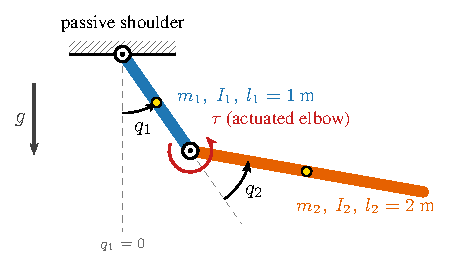
\includegraphics[width=0.56\columnwidth]{acrobot_diagram.pdf}
\caption{Acrobot schematic (to scale); dots mark the centres of mass.}\label{fig:schematic}
\end{figure}

\subsection{Given Equations of Motion}
\begin{equation}
M(q)\ddot q+C(q,\dot q)\dot q=\tau_g(q)+B\tau,\qquad B=\begin{bmatrix}0\\1\end{bmatrix}\label{eq:eom}
\end{equation}
($B$ applies $\tau$ to the elbow equation only.) Below we derive each term with $c_2=\cos q_2$, $s_2=\sin q_2$.

\subsection{Derivation}
\textit{1) Potential energy and gravity torque:}
\begin{align}
U&=-(m_1l_{c1}+m_2l_1)\,g\cos q_1-m_2l_{c2}\,g\cos\varphi\nonumber\\
&=-14.715\cos q_1-9.81\cos\varphi,\nonumber\\
\tau_g&=-\frac{\partial U}{\partial q}=-9.81\begin{bmatrix}1.5\sin q_1+\sin\varphi\\ \sin\varphi\end{bmatrix}.\label{eq:tg}
\end{align}

\textit{2) Kinetic energy and inertia matrix:} the velocity of centre~2 is the elbow velocity ($l_1\dot q_1$) plus the rotation about the elbow ($l_{c2}\dot\varphi$), at angle $q_2$ apart (law of cosines):
\begin{align*}
T&=\tfrac12(m_1l_{c1}^2+I_1)\dot q_1^2+\tfrac12I_2\dot\varphi^2\\
&\quad+\tfrac12m_2\big(l_1^2\dot q_1^2+l_{c2}^2\dot\varphi^2+2l_1l_{c2}c_2\dot q_1\dot\varphi\big)=\tfrac12\dot q^TM\dot q,
\end{align*}
\begin{equation}
M(q)=\begin{bmatrix}2.663+2c_2 & 1.33+c_2\\ 1.33+c_2 & 1.33\end{bmatrix}.\label{eq:M}
\end{equation}

\textit{3) Coriolis term (Euler--Lagrange):}
\begin{align*}
&\frac{d}{dt}\frac{\partial T}{\partial\dot q}-\frac{\partial T}{\partial q}=\tau_g+B\tau,\qquad \frac{\partial T}{\partial\dot q}=M\dot q\\
&\Rightarrow\; M\ddot q+\underbrace{\Big(\dot M\dot q-\frac{\partial T}{\partial q}\Big)}_{=\,C\dot q}=\tau_g+B\tau .
\end{align*}
With $\dot M=\frac{\partial M}{\partial q_2}\dot q_2=-s_2\dot q_2\left[\begin{smallmatrix}2&1\\1&0\end{smallmatrix}\right]$ this evaluates to
\begin{equation}
C(q,\dot q)=s_2\begin{bmatrix}-2\dot q_2 & -\dot q_2\\ \dot q_1 & 0\end{bmatrix}.\label{eq:C}
\end{equation}
These are the same $\tau_g$, $M$ and $C$ as in the given model.

\subsection{State-Space Form}
\begin{align}
\det M&=(2.663+2c_2)(1.33)-(1.33+c_2)^2\nonumber\\
&=1.7729-c_2^2\;\ge\;0.7729>0\quad(c_2^2\le1),\nonumber\\
\dot x&=f(x,\tau)=\begin{bmatrix}\dot q\\ M^{-1}\big(\tau_g+B\tau-C\dot q\big)\end{bmatrix}.\label{eq:f}
\end{align}

% =====================================================================
\section{Equilibria}
% =====================================================================
\subsection{Conditions}
At rest $\dot q=\ddot q=0$, and the input torque is given as $\tau^*=0$. Then~\eqref{eq:eom} gives $\tau_g(q^*)=0$:
\begin{align*}
\text{row 2:}\quad&\sin(q_1^*+q_2^*)=0,\\
\text{row 1:}\quad&1.5\sin q_1^*+\underbrace{\sin(q_1^*+q_2^*)}_{=0}=0\;\Rightarrow\;\sin q_1^*=0 .
\end{align*}

\subsection{Solutions}
\begin{equation*}
q_1^*\in\{0,\pi\},\quad q_1^*+q_2^*\in\{0,\pi\}\;\Rightarrow\;q_2^*\in\{0,\pi\}\pmod{2\pi}.
\end{equation*}
$\Rightarrow$ \textbf{four equilibria} (Table~\ref{tab:eq}), all with both links vertical.

\begin{table}[h]
\caption{Equilibria for $\tau^*=0$}\label{tab:eq}
\centering\footnotesize\setlength{\tabcolsep}{4pt}
\begin{tabular}{@{}clcrl@{}}
\toprule
 & Posture & $(q_1^*,q_2^*)$ & $U$ [J] & Description\\
\midrule
$E_1$ & down--down & $(0,0)$ & $-24.525$ & both links hanging\\
$E_2$ & down--up & $(0,\pi)$ & $-4.905$ & link 1 down, link 2 up\\
$E_3$ & up--up & $(\pi,0)$ & $+24.525$ & fully upright (target)\\
$E_4$ & up--down & $(\pi,\pi)$ & $+4.905$ & link 1 up, link 2 down\\
\bottomrule
\end{tabular}
\end{table}

% ---------- wide table ----------
\begin{table*}[t]
\caption{Transfer functions $G_i(s)=N_i(s)/\Delta(s)$ at the four equilibria}\label{tab:tf}
\centering\footnotesize\setlength{\tabcolsep}{5pt}\renewcommand{\arraystretch}{1.15}
\begin{tabular}{@{}cllllll@{}}
\toprule
 & Denominator $\Delta(s)$ (monic) & $N_1(s)$ \;($\tau\to q_1$) & $N_2(s)$ \;($\tau\to q_2$) & Poles & Zeros of $G_1$ & Zeros of $G_2$\\
\midrule
$E_1$ & $s^4+42.2410\,s^2+186.7719$ & $-3.0147\,(s^2+4.2103)$ & $6.0332\,(s^2+5.2595)$ & $\pm j2.2400,\ \pm j6.1011$ & $\pm j2.0519$ & $\pm j2.2934$\\
$E_2$ & $s^4+8.4025\,s^2-186.7719$ & $-0.4270\,(s^2-29.7273)$ & $0.8578\,(s^2+7.3982)$ & $\pm3.1775,\ \pm j4.3010$ & $\pm5.4523$ & $\pm j2.7200$\\
$E_3$ & $s^4-42.2410\,s^2+186.7719$ & $-3.0147\,(s^2-4.2103)$ & $6.0332\,(s^2-5.2595)$ & $\pm2.2400,\ \pm6.1011$ & $\pm2.0519$ & $\pm2.2934$\\
$E_4$ & $s^4-8.4025\,s^2-186.7719$ & $-0.4270\,(s^2+29.7273)$ & $0.8578\,(s^2-7.3982)$ & $\pm4.3010,\ \pm j3.1775$ & $\pm j5.4523$ & $\pm2.7200$\\
\bottomrule
\end{tabular}
\end{table*}

\newpage
% =====================================================================
\section{Linearization}
% =====================================================================
\subsection{Deviation Variables}
\begin{equation*}
\tilde q=\begin{bmatrix}q_1-q_1^*\\ q_2-q_2^*\end{bmatrix},\quad
\tilde x=\begin{bmatrix}\tilde q\\ \dot{\tilde q}\end{bmatrix}=x-x^*,\quad
\tilde\tau=\tau-\tau^*=\tau .
\end{equation*}
First-order Taylor expansion of~\eqref{eq:f} about $(x^*,0)$:
\begin{equation*}
\dot{\tilde x}\approx\underbrace{f(x^*,0)}_{=0}+\frac{\partial f}{\partial x}\Big|_*\tilde x+\frac{\partial f}{\partial\tau}\Big|_*\tilde\tau .
\end{equation*}

\subsection{Jacobians}
\textit{Top half:} $\tfrac{d}{dt}\tilde q=\dot{\tilde q}$ $\Rightarrow$ rows $[\,0\;\;I_2\,]$.

\textit{Bottom half:} $h=M^{-1}(\tau_g+B\tau-C\dot q)$. At $(x^*,0)$:
\begin{align*}
\partial(C\dot q)/\partial\dot q&=0 &&(C\dot q\text{ is quadratic in }\dot q,\ \dot q^*=0)\\
(\partial M^{-1}/\partial q)(\tau_g+B\tau)&=0 &&(\tau_g(q^*)=0,\ \tau^*=0)
\end{align*}
\begin{equation*}
\Rightarrow\;\ddot{\tilde q}=P\tilde q+r\tilde\tau,\qquad P=M(q^*)^{-1}K(q^*),\quad r=M(q^*)^{-1}B,
\end{equation*}
\begin{equation}
K(q^*)=\frac{\partial\tau_g}{\partial q}\Big|_{q^*}=-9.81\begin{bmatrix}1.5\cos q_1^*+\cos\varphi^* & \cos\varphi^*\\ \cos\varphi^* & \cos\varphi^*\end{bmatrix}.\label{eq:K}
\end{equation}

\subsection{Linear State-Space Model}
Stacking both halves, with the joint angles as outputs, $y=\tilde q=[q_1-q_1^*,\;q_2-q_2^*]^T$:
\begin{equation}
\boxed{\begin{aligned}
\dot{\tilde x}&=A\tilde x+B_\ell\tilde\tau,\qquad y=C_y\tilde x+D\tilde\tau,\\
A&=\begin{bmatrix}0 & I_2\\ P & 0\end{bmatrix}\!,\;
B_\ell=\begin{bmatrix}0\\ r\end{bmatrix}\!,\;
C_y=\begin{bmatrix}I_2 & 0\end{bmatrix}\!,\; D=0
\end{aligned}}\label{eq:AB}
\end{equation}

\subsection{Example: $E_1=(0,0)$}
$\cos q_1^*=\cos\varphi^*=c_2=1$:
\begin{gather*}
K=\begin{bmatrix}-24.525&-9.81\\-9.81&-9.81\end{bmatrix}\!,\quad
M=\begin{bmatrix}4.663&2.33\\2.33&1.33\end{bmatrix}\!,\\
\det M=0.7729,\qquad M^{-1}=\frac{1}{0.7729}\begin{bmatrix}1.33&-2.33\\-2.33&4.663\end{bmatrix}\!,\\
P_{E1}=M^{-1}K=\begin{bmatrix}-12.6292&12.6926\\14.7488&-29.6119\end{bmatrix}\!,\quad
r_{E1}=\begin{bmatrix}-3.0147\\6.0332\end{bmatrix}\!.
\end{gather*}

\subsection{All Equilibria}
$M$ depends only on $q_2^*$; $K$ only on the signs of $\cos q_1^*$, $\cos\varphi^*$. Upside down, gravity flips:
\begin{equation*}
K_{E3}=-K_{E1},\;M_{E3}=M_{E1}\Rightarrow P_{E3}=-P_{E1};\qquad P_{E4}=-P_{E2}.
\end{equation*}
Results in Table~\ref{tab:lin}; with~\eqref{eq:AB} they give $(A,B_\ell,C_y,D)$ at each equilibrium.

\begin{table}[h]
\caption{Linearization results ($\det M=0.7729$ at all four)}\label{tab:lin}
\centering\footnotesize\setlength{\tabcolsep}{4pt}\renewcommand{\arraystretch}{1.3}
\begin{tabular}{@{}ccccc@{}}
\toprule
 & $(\cos q_1^*,\cos\varphi^*)$ & $M(q^*)$ & $P=M^{-1}K$ & $r=M^{-1}B$\\
\midrule
$E_1$ & $(1,1)$ & $\left[\begin{smallmatrix}4.663&2.33\\2.33&1.33\end{smallmatrix}\right]$ & $\left[\begin{smallmatrix}-12.6292&12.6926\\14.7488&-29.6119\end{smallmatrix}\right]$ & $\left[\begin{smallmatrix}-3.0147\\6.0332\end{smallmatrix}\right]$\\
$E_2$ & $(1,-1)$ & $\left[\begin{smallmatrix}0.663&0.33\\0.33&1.33\end{smallmatrix}\right]$ & $\left[\begin{smallmatrix}-12.6292&12.6926\\10.5095&4.2266\end{smallmatrix}\right]$ & $\left[\begin{smallmatrix}-0.4270\\0.8578\end{smallmatrix}\right]$\\
$E_3$ & $(-1,-1)$ & as $E_1$ & $-P_{E1}$ & $r_{E1}$\\
$E_4$ & $(-1,1)$ & as $E_2$ & $-P_{E2}$ & $r_{E2}$\\
\bottomrule
\end{tabular}
\end{table}

% =====================================================================
\section{Transfer Functions}
% =====================================================================
\subsection{Laplace Transform}
Define $\tilde Q_i(s)=\mathcal L\{\tilde q_i(t)\}$, $\tilde{\mathcal T}(s)=\mathcal L\{\tilde\tau(t)\}$, $\tilde Q=[\tilde Q_1,\tilde Q_2]^T$. With zero initial conditions ($\ddot{\tilde q}\to s^2\tilde Q$):
\begin{equation*}
s^2\tilde Q=P\tilde Q+r\tilde{\mathcal T}\;\Rightarrow\;(s^2I-P)\,\tilde Q(s)=r\,\tilde{\mathcal T}(s).
\end{equation*}

\subsection{General Formula}
\begin{gather*}
(s^2I-P)^{-1}=\frac{1}{\Delta(s)}\begin{bmatrix}s^2-P_{22}&P_{12}\\P_{21}&s^2-P_{11}\end{bmatrix},\\
\Delta(s)=\det(s^2I-P)=s^4-\operatorname{tr}(P)\,s^2+\det P .
\end{gather*}
Multiplying by $r$ and dividing each row by $\tilde{\mathcal T}$ ($G_i=\tilde Q_i/\tilde{\mathcal T}$):
\begin{equation}
\boxed{\begin{aligned}
G_1(s)&=\frac{r_1s^2+(P_{12}r_2-P_{22}r_1)}{\Delta(s)},\\[2pt]
G_2(s)&=\frac{r_2s^2+(P_{21}r_1-P_{11}r_2)}{\Delta(s)}
\end{aligned}}\label{eq:G}
\end{equation}
\begin{itemize}
\item \textit{Poles:} roots of $\Delta$ (= eigenvalues of $A$); with $\lambda=s^2$, $\lambda^2-\operatorname{tr}(P)\lambda+\det P=0$, then $s=\pm\sqrt\lambda$.
\item \textit{Zeros:} roots of the numerators, $s^2=-(P_{12}r_2-P_{22}r_1)/r_1$ and $s^2=-(P_{21}r_1-P_{11}r_2)/r_2$.
\end{itemize}

\subsection{Example: $E_1$}
\begin{align*}
\operatorname{tr}P&=-42.2410,\quad \det P=186.7719\\
\Rightarrow\Delta&=s^4+42.2410\,s^2+186.7719,\\
\lambda&=\tfrac{-42.2410\pm32.206}{2}=-5.018,\;-37.224\\
\Rightarrow\text{poles}&=\pm j2.2400,\;\pm j6.1011,\\
P_{12}r_2-P_{22}r_1&=-12.6926,\quad P_{21}r_1-P_{11}r_2=31.7316,
\end{align*}
\begin{equation*}
G_1=\frac{-3.0147(s^2+4.2103)}{\Delta(s)},\qquad G_2=\frac{6.0332(s^2+5.2595)}{\Delta(s)} .
\end{equation*}

\subsection{Results}
Table~\ref{tab:tf} lists all four equilibria. With no friction only even powers of $s$ occur, so poles and zeros come in pairs $\pm p$; since $P_{E3}=-P_{E1}$, each $\pm j\omega$ at $E_1$ becomes $\pm\omega$ at $E_3$ (likewise $E_2$/$E_4$).

\newpage
% =====================================================================
\section{Verification}
% =====================================================================
\begin{itemize}
\item The model derivation and all values in Tables~\ref{tab:tf} and~\ref{tab:lin} were verified in MATLAB (agreement to four decimals).
\item Nonlinear~\eqref{eq:f} vs.\ linear~\eqref{eq:AB}, simulated in Python from the same small deviation, $\tau=0$ (Fig.~\ref{fig:sim}): near $E_1$ from $\tilde q(0)=(0.1,-0.1)$~rad they agree within $1.0^\circ$ ($q_1$) and $2.0^\circ$ ($q_2$) over 8~s; near $E_3$ from $\tilde q_1(0)=10^{-3}$~rad the error is $0.02\%$ at $|\tilde q_1|=1^\circ$.
\item With $\tau=0$, $T+U$ stays constant to $10^{-8}$ (no friction).
\item \textbf{Animation} (Manim) of the model, the four equilibria, the nonlinear vs.\ linear responses near each equilibrium and the pole--zero maps: \href{https://drive.google.com/file/d/18Ic6QdsY37QBfvFIwmVA_8Z-u4AyNPdg/view?usp=sharing}{\textcolor{blue!60!black}{\textbf{watch the video}}}\\
{\footnotesize\urlstyle{same}\textcolor{blue!60!black}{\url{https://drive.google.com/file/d/18Ic6QdsY37QBfvFIwmVA_8Z-u4AyNPdg/view?usp=sharing}}}
\end{itemize}

\begin{figure}[!h]
\centering
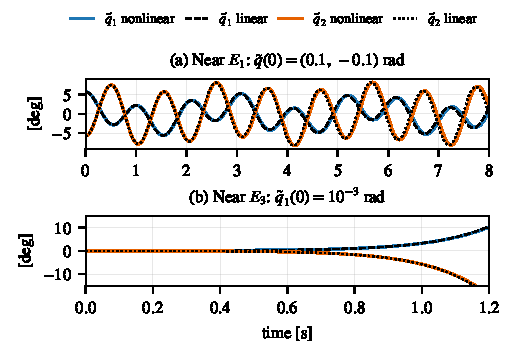
\includegraphics[width=0.9\columnwidth]{sim.pdf}
\caption{Free responses of the nonlinear (colour) and linear (black) models near (a) $E_1$ and (b) $E_3$ (simulated in Python).}\label{fig:sim}
\end{figure}

{\footnotesize
\begin{thebibliography}{9}\setlength{\itemsep}{0pt}
\bibitem{spong95} M.~W. Spong, ``The swing up control problem for the Acrobot,'' \emph{IEEE Control Syst. Mag.}, vol.~15, no.~1, pp.~49--55, 1995.
\bibitem{tedrake} R.~Tedrake, \emph{Underactuated Robotics}, MIT, 2024. [Online]. Available: https://underactuated.csail.mit.edu
\end{thebibliography}}

\end{document}
